\documentclass[a4paper]{article}

%% Language and font encodings
\usepackage[french]{babel}
\usepackage[utf8x]{inputenc}
\usepackage[T1]{fontenc}




%% Sets page size and margins
\usepackage[a4paper,top=3cm,bottom=2cm,left=3cm,right=3cm,marginparwidth=1.75cm]{geometry}
\usepackage{mathtools, bm}
\usepackage{amssymb, bm}
\usepackage{listings}

% \renewcommand{\thesection}{\arabic{section})}
% \renewcommand{\thesubsection}{\alph{subsection})}


%% Useful packages
\usepackage{amsmath}
\usepackage{graphicx}
\usepackage[colorinlistoftodos]{todonotes}
\usepackage[colorlinks=true, allcolors=black]{hyperref}

\usepackage{algorithm2e}
\usepackage[section]{placeins}

\title{
    \begin{minipage}\linewidth
        \centering\bfseries\sffamily
        TP - Évaluation des performances par mesure
    \end{minipage}}
\author{Maxime Kermarquer - M2 CHPS}
\date{}

\begin{document}
\maketitle

VDbench est un générateur d'entrée/sortie sur disque, utilisé pour testé et évaluer des produits de stockage.
Le but de ce TP était de nous familiariser avec cette outil de mesure, et de pouvoir exploiter les mesures obtenues. L'ensemble des mesures ont été prises sur un disque dur Western Digital Caviar Green (AF) de 2 To fonctionnant à 7 200 tr/min.\\
J'ai utilisé le langage R pour réaliser des statistiques sur les mesures et gnuplot pour tracer les histogrammes.

\section{Expérimentations : Visualisation des résultats}

J'ai organisé mon TP, avec un dossier pour chaque question, chacun contenant :
\begin{itemize}
\item Un \textbf{Makefile} pour exécuter les scripts et visualiser les résultats.
\item Un dossier \textbf{DATA} qui contient les mesures.
\item Un dossier \textbf{SCRIPT\_R} qui contient le script R permettant de calculer des statistiques sur les mesures.
\item Un dossier \textbf{RESULTATS} qui contient les statistiques des mesures dans plusieurs fichiers \emph{.txt}.
\item Un dossier \textbf{SCRIPT\_GNUPLOT} qui contient les scripts gnuplot pour tracer les histogrammes sur le temps de réponse et la bande-passante.
\item Un dossier \textbf{PLOT} qui contient les histogrammes générés au format \emph{.eps}.
\end{itemize}

\begin{figure}[h]
	\begin{center}
		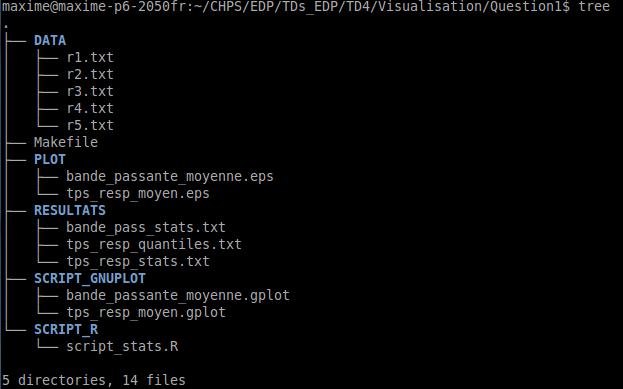
\includegraphics[scale=0.55]{SCREEN/arborescence.png}
	\end{center}
   	\caption{Arborescence du TP}
	\label{fig:arbo}
\end{figure}

\FloatBarrier

\subsection*{Utilisation du Makefile}
Le \textbf{Makefile} a plusieurs règles : 
\begin{itemize}
\item \textbf{make clean} supprime les graphiques.
\item \textbf{make clean\_stats} supprime les statistiques des mesures.
\item \textbf{make stats} exécute le script R pour générer les statistiques.
\item \textbf{make} exécute les scripts gnuplot pour générer les histogrammes.
\item \textbf{make visu} pour visualiser les histogrammes.
\end{itemize}

% \begin{figure}[h]
% 	\begin{center}
% 		\lstinputlisting{CODE/Makefile}
% 	\end{center}
%    	\caption{Makefile}
% 	\label{fig:makefile}
% \end{figure}

% \FloatBarrier


\subsection{Question 1}

Pour visualiser les quantiles du temps de réponse, on doit se placer dans le dossier de la question et utiliser la commande : \\
\textbf{cat RESULTATS/tps\_resp\_quantiles.txt}

\begin{itemize}
\item La colonne 1 correspond à l'exécution.
\item La colonne 2 au premier quartile.
\item La colonne 3 au second quartile.
\item La colonne 4 au troisième quartile.
\end{itemize}

\begin{figure}[h]
	\begin{center}
		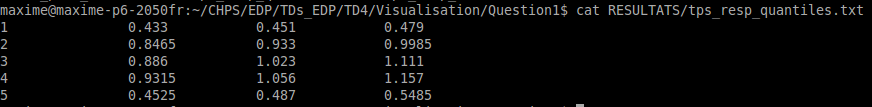
\includegraphics[scale=0.55]{SCREEN/quantiles.png}
	\end{center}
   	\caption{Affichage des quantiles}
	\label{fig:quantiles}
\end{figure}

\FloatBarrier


\subsection{Question 2}

Pour visualiser l'évolution du temps de réponse en fonction de l'exécution, j'ai choisi de calculer la moyenne de celui-ci pour l'exécution donnée et de l'afficher sous forme d'histogramme. Un exemple de script de visualisation est donné en annexe dans la figure \ref{fig:scriptGnuplot2}.


\subsection{Question 3}

Comme pour le temps de réponse, je calcule la moyenne de la bande-passante pour l'exécution, et j'affiche les moyennes obtenus sous forme d'histogramme.
Un exemple est aussi donné en annexe dans la figure \ref{fig:scriptGnuplot}.

\subsection{Question 4}

Pour visualiser les statistiques du temps de réponse, on doit se placer dans le dossier de la question 3 et utiliser la commande : \\
\textbf{cat RESULTATS/tps\_resp\_stats.txt}

\begin{itemize}
\item La colonne 1 correspond à l'exécution.
\item La colonne 2 à la moyenne.
\item La colonne 3 à la variance.
\item La colonne 4 à la borne inférieure de l'intervalle de confiance.
\item La colonne 5 à la borne supérieure de l'intervalle de confiance.
\end{itemize}

\begin{figure}[h]
	\begin{center}
		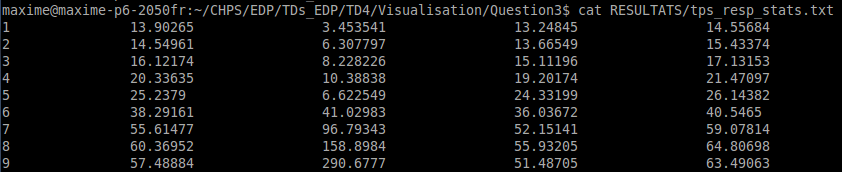
\includegraphics[scale=0.55]{SCREEN/stats.png}
	\end{center}
   	\caption{Affichage des statistiques du temps de réponse}
	\label{fig:quantiles}
\end{figure}

\FloatBarrier


\newpage
\section{Expérimentations : Variations des paramètres}

\subsection{Question 1 : Accès séquentiel}

\begin{figure}[h]
	\begin{center}
		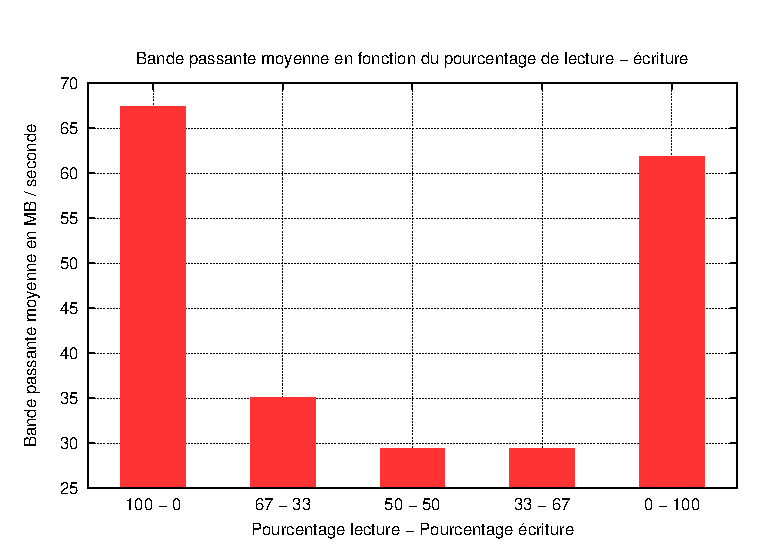
\includegraphics[scale=0.70]{Question1/bande_passante_moyenne.eps}
	\end{center}
   	\caption{Évolution de la bande-passante en fonction du pourcentage de lecture en accès séquentiel}
	\label{fig:courbe_bande_passante_lect_seq}
\end{figure}

\FloatBarrier

\begin{figure}[h]
	\begin{center}
		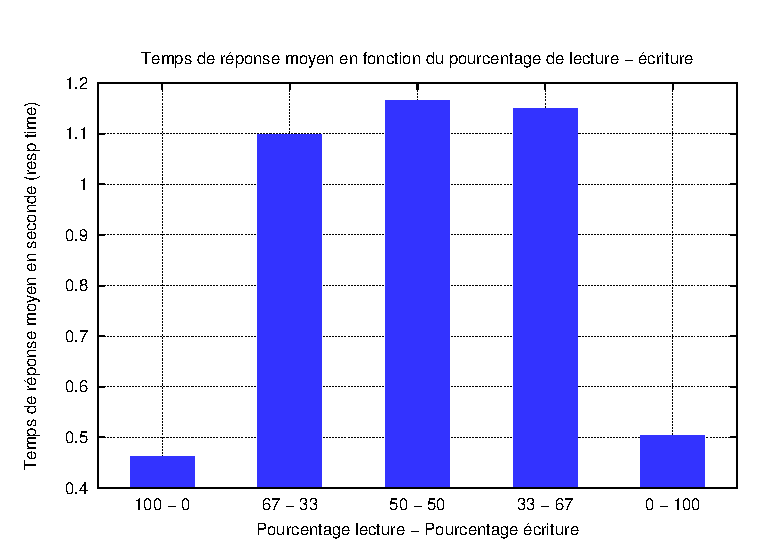
\includegraphics[scale=0.70]{Question1/tps_resp_moyen.eps}
	\end{center}
   	\caption{Évolution du temps de réponse en fonction du pourcentage de lecture en accès séquentiel}
	\label{fig:courbe_tps_rep_lect_seq}
\end{figure}
\FloatBarrier

On peut observer qu'on obtient de meilleures performances (temps de réponse petit, débit élevé) en réalisant uniquement des lectures, ou uniquement des écritures.\\


\newpage
\subsection{Question 2 : Accès aléatoire}

\begin{figure}[h]
	\begin{center}
		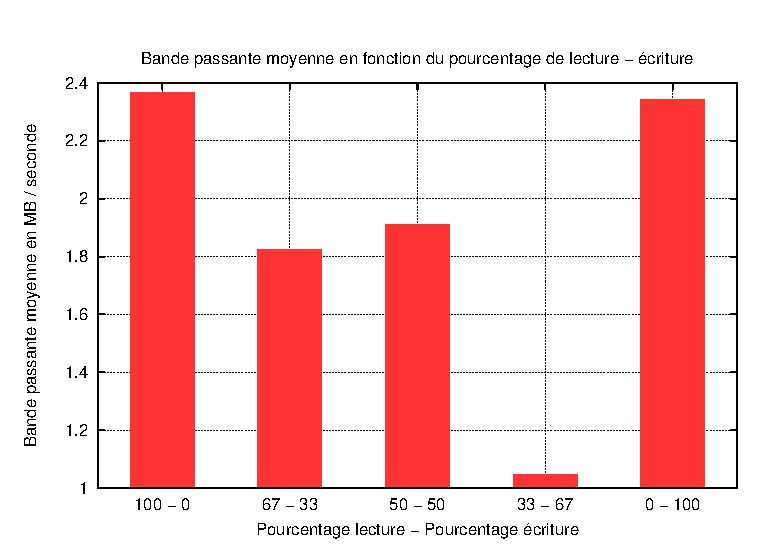
\includegraphics[scale=0.70]{Question2/bande_passante_moyenne.eps}
	\end{center}
   	\caption{Évolution de la bande passante en fonction du pourcentage de lecture en accès aléatoire}
	\label{fig:courbe_bande_passante_lect_alea}
\end{figure}

\FloatBarrier

\begin{figure}[h]
	\begin{center}
		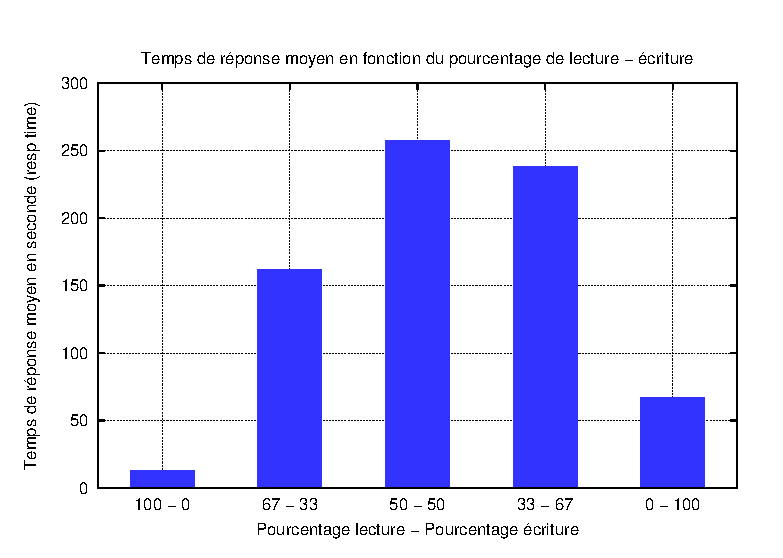
\includegraphics[scale=0.70]{Question2/tps_resp_moyen.eps}
	\end{center}
   	\caption{Évolution du temps de réponse en fonction du pourcentage de lecture en accès aléatoire}
	\label{fig:courbe_tps_rep_lect_alea}
\end{figure}

\FloatBarrier

Comme pour l'accès séquentiel, on peut observer qu'on obtient de meilleures performances en réalisant uniquement des lectures, ou uniquement des écritures, bien que cela soit moins marqué.\\
On note sur la figure \ref{fig:courbe_bande_passante_lect_alea} pour l'exécution avec avec 33\% de lecture et 67\% d'écriture une bande-passante très faible. Cela est sûrement dû à une erreur de mesure. 


\newpage
\subsection{Question 3 - Taille des requêtes}

\begin{figure}[h]
	\begin{center}
		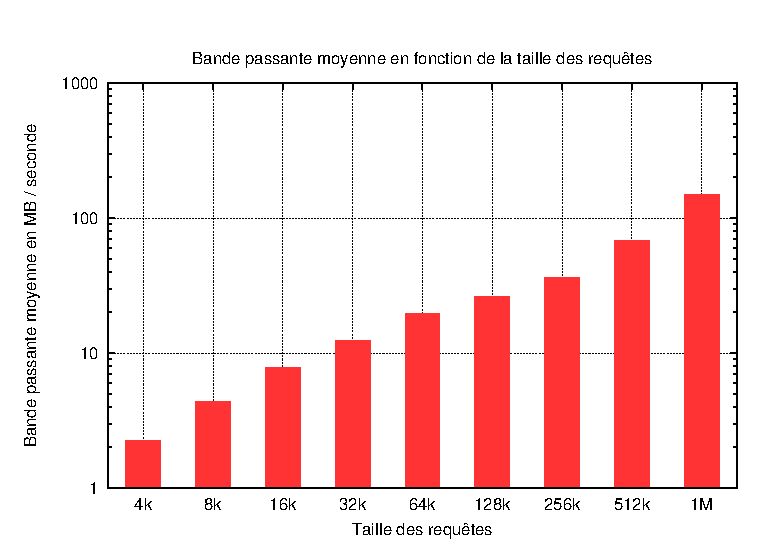
\includegraphics[scale=0.70]{Question3/bande_passante_moyenne.eps}
	\end{center}
   	\caption{Évolution de la bande passante en fonction de la taille des requêtes}
	\label{fig:courbe_bande_passante_taille}
\end{figure}

\FloatBarrier

\begin{figure}[h]
	\begin{center}
		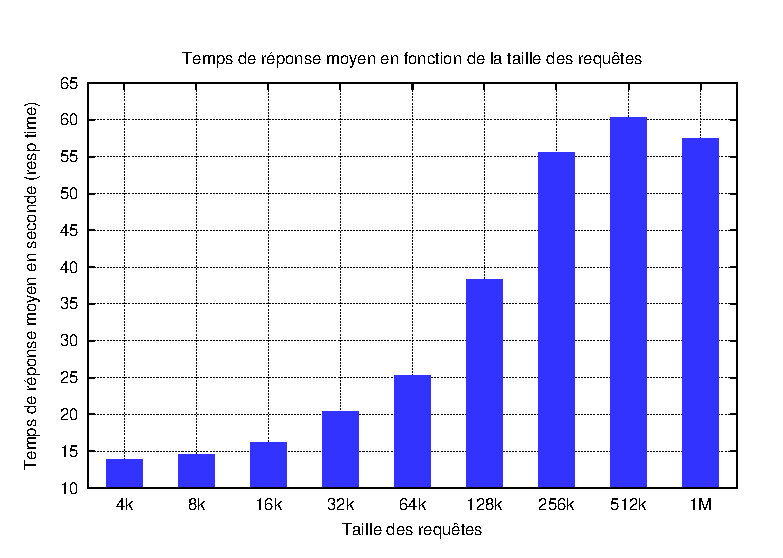
\includegraphics[scale=0.70]{Question3/tps_resp_moyen.eps}
	\end{center}
   	\caption{Évolution du temps de réponse en fonction de la taille des requêtes}
	\label{fig:courbe_tps_rep_taille}
\end{figure}

\FloatBarrier

Sur l'histogramme figure \ref{fig:courbe_bande_passante_taille}, j'ai utilisé une échelle logarithmique. \\
On observe que la bande-passante augmente avec la taille des requêtes. 
L'ensemble des statistiques sur le temps de réponse sont données dans la table \ref{tab:stats_tps_reponse}.


\begin{table}[htbp!]
  \centerline{
    \begin{tabular}{|c|c|c|c|}
      \hline	
	Taille des requête & Moyenne & Variance & Intervalle de confiance\\
      \hline\hline
        4KB		&	13.90265	&	3.453541	&	[13.24845	,	14.55684]	\\
        8KB		&	14.54961	&	6.307797	&	[13.66549	,	15.43374]	\\
        16KB	&	16.12174	&	8.228226	&	[15.11196	,	17.13153]	\\
        32KB	&	20.33635	&	10.38838	&	[19.20174	,	21.47097]	\\
        64KB	&	25.2379		&	6.622549	&	[24.33199	,	26.14382]	\\
        128KB	&	38.29161	&	41.02983	&	[36.03672	,	40.5465]	\\
        256KB	&	55.61477	&	96.79343	&	[52.15141	,	59.07814]	\\
        512KB	&	60.36952	&	158.8984	&	[55.93205	,	64.80698]	\\
        1MB		&	57.48884	&	290.6777	&	[51.48705	,	63.49063]	\\
      \hline
    \end{tabular}
  }
  \caption{Statistiques sur le temps de réponse.}
  \label{tab:stats_tps_reponse}
\end{table}

\newpage
\subsection{Question 4 - Nombres de threads}

\begin{figure}[h]
	\begin{center}
		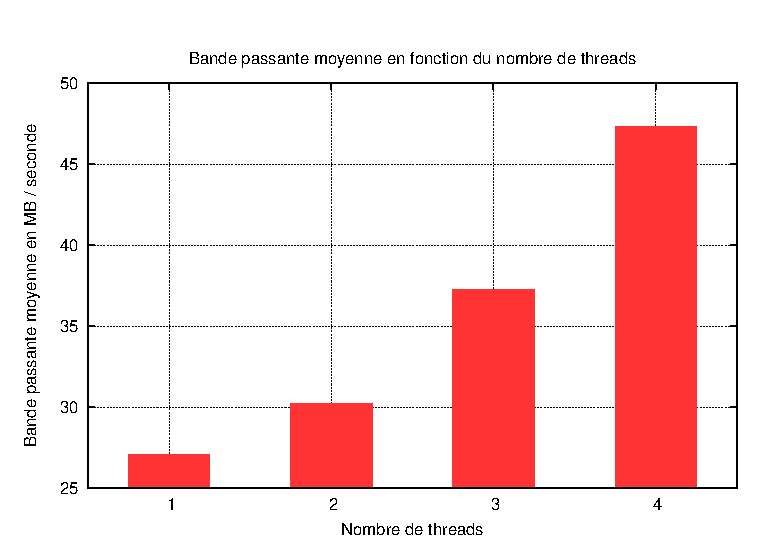
\includegraphics[scale=0.70]{Question4/bande_passante_moyenne.eps}
	\end{center}
   	\caption{Évolution de la bande passante en fonction du nombre de threads}
	\label{fig:courbe_bande_passante_thread}
\end{figure}

\FloatBarrier

\begin{figure}[h]
	\begin{center}
		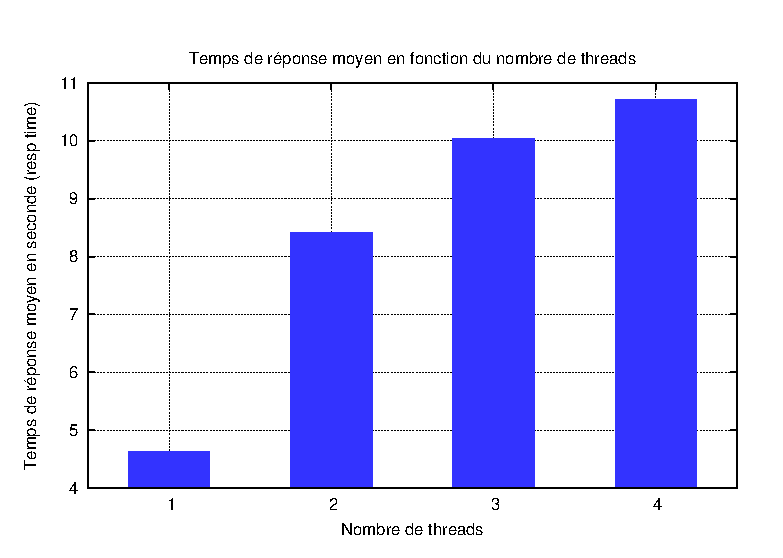
\includegraphics[scale=0.70]{Question4/tps_resp_moyen.eps}
	\end{center}
   	\caption{Évolution du temps de réponse en fonction du nombre de threads}
	\label{fig:courbe_tps_rep_thread}
\end{figure}

\FloatBarrier

On observe que le temps de réponse et la bande-passante augmentent avec le nombre de threads en parallèle.


\newpage
\appendix

\section{Scripts de visualisation}
\begin{figure}[h]
	\begin{center}
		\lstinputlisting[language=bash]{CODE/gnuplot2.txt}
	\end{center}
   	\caption{Exemple de script de visualisation Gnuplot pour le temps de réponse}
	\label{fig:scriptGnuplot2}
\end{figure}

\begin{figure}[h]
	\begin{center}
		\lstinputlisting[language=bash]{CODE/gnuplot.txt}
	\end{center}
   	\caption{Exemple de script de visualisation Gnuplot pour la bande-passante}
	\label{fig:scriptGnuplot}
\end{figure}

\FloatBarrier

\FloatBarrier

% \lstinputlisting[language=C]{CODE/script_stats.R}
% \caption{Exemple de script R calculant les différentes statistiques des résultats}
% \label{fig:script_r}




\end{document}